\documentclass[11pt,professionalfont,aspectratio=43]{beamer}

% Assets
\usepackage[czech]{babel}				% Jazyk
\usepackage[a-2u]{pdfx}				    % Kopírování z pdfka
\usepackage{tikz}						% Schémata automatů
\usetikzlibrary{shadows, shadows.blur, shapes.geometric, arrows, positioning, overlay-beamer-styles, patterns, shadings, shapes.callouts}
% \usetikzlibrary{arrows}
\usepackage{pgfplots}
% \pgfplotsset{compat=1.15}
% \usepackage{mathrsfs}
\usepackage[export]{adjustbox}

\usepackage[T1]{fontenc}
\usefonttheme[onlymath]{serif}
% \usepackage{newtxmath}
\usepackage{pxfonts}
\usepackage{slantsc}
% \usepackage{varwidth}

\usepackage[linesnumbered,ruled,vlined]{algorithm2e}                % Pseudokód algoritmů
\usepackage[utf8]{inputenc}
% \usepackage{textcomp}
\usepackage{hyperref}
\usepackage{fancybox}

%%% FONTS
% \usefonttheme{serif}
% \usepackage{lmodern}
\usepackage{helvet}

\hypersetup{%
    pdfencoding=auto,
    pdfauthor={\insertauthor},
    pdftitle={\insertsubtitle}
}
\usepackage{float}
\usepackage{csquotes}					% české uvozovky
\usepackage{enumerate}					% enumerate environment
\usepackage{indentfirst}
\usepackage{tcolorbox}                  % Fancy boxíky
\usepackage{mathtools}
\usepackage{pifont}
\usepackage{cancel}
\usepackage{subcaption}
\usepackage{soul}
\usepackage{makecell}                   % Zalomení v buňce tabulky
\usepackage{xcolor}
\usepackage{graphicx}
\usepackage{tabularx}
\usepackage{amsmath}
\usepackage{amsthm}
\usepackage{colortbl}                   % Barvení buněk v tabulce
\usepackage{multicol}                   % Rozdělení obsahu do sloucpů

\usepackage{listings}                   % Úryvky z kódu
\definecolor{maroon}{rgb}{0.5,0,0}
\definecolor{forestgreen}{rgb}{0.13, 0.55, 0.13}

% \lstdefinelanguage{XML}
% {
%   basicstyle=\ttfamily,
%   morestring=[s]{"}{"},
%   morecomment=[s]{?}{?},
%   morecomment=[s]{!--}{--},
%   commentstyle=\color{forestgreen},
%   moredelim=[s][\color{black}]{>}{<},
%   moredelim=[s][\color{red}]{\ }{=},
%   stringstyle=\color{blue},
%   identifierstyle=\color{maroon}
% }
% Colors

\def\maincolR{0} % červená složka (0–255)
\def\maincolG{83} % zelená složka
\def\maincolB{120} % modrá složka
\definecolor{maincolor}{HTML}{8B00B5}

% \pgfmathtruncatemacro{\authorfooterbgR}{1*\maincolR}
% \pgfmathtruncatemacro{\authorfooterbgG}{1*\maincolG}
% \pgfmathtruncatemacro{\authorfooterbgB}{1*\maincolB}
% \definecolor{authorfooterbg}{RGB}{\authorfooterbgR,\authorfooterbgG,\authorfooterbgB}

% \pgfmathtruncatemacro{\titlefooterbgR}{0.722*\maincolR}   
% \pgfmathtruncatemacro{\titlefooterbgG}{0.974*\maincolG}   
% \pgfmathtruncatemacro{\titlefooterbgB}{0.739*\maincolB}
% \definecolor{titlefooterbg}{RGB}{\titlefooterbgR,\titlefooterbgG,\titlefooterbgB}

% Beamer theme
\colorlet{themecolor}{maincolor}
\colorlet{authorfooterbg}{maincolor}
\definecolor{titlefooterbg}{HTML}{9471B0}
\definecolor{titlefooterfg}{HTML}{000000}
\colorlet{titlecolorfg}{maincolor}
\definecolor{titleboxbg}{HTML}{E7E7E7}
\definecolor{datefooterbg}{HTML}{E3E3E3}
\colorlet{titleframeboxcolor}{maincolor}

% Background gradient
\definecolor{gradMiddle}{RGB}{212,248,255}
\definecolor{gradEnd}{RGB}{114,231,255}

% Block theme
\definecolor{blocktitlebg}{HTML}{F0DFA9}
\definecolor{blocktitlefg}{HTML}{957300}
\definecolor{blockbodybg}{HTML}{F5F0DF}

\definecolor{alertblockbodybg}{HTML}{FFE4E4}
\definecolor{alertblocktitlebg}{HTML}{ECA4A4}
\definecolor{alertblocktitlefg}{HTML}{B11313}

\definecolor{exampleblockbodybg}{HTML}{DAF0DA}
\definecolor{exampleblocktitlebg}{HTML}{BBE0BB}
\definecolor{exampleblocktitlefg}{HTML}{257A25}

\definecolor{mathfg}{HTML}{00185E}

\colorlet{bulletbg}{maincolor}
% \definecolor{bulletbg}{HTML}{}

% Beamer theme
\usetheme{Madrid}
\usecolortheme{seahorse}
% \useoutertheme[subsection=false]{miniframes}

\usecolortheme[named=themecolor]{structure}
\setbeamertemplate{frame numbering}[fraction]
\setbeamertemplate{navigation symbols}{}
\setbeamercovered{invisible}

% Header/footer
\setbeamercolor{author in head/foot}{bg=authorfooterbg,fg=white}
\setbeamercolor{title in head/foot}{bg=titlefooterbg,fg=titlefooterfg}
\setbeamercolor{date in head/foot}{bg=datefooterbg,fg=black}
% \setbeamercolor{title}{bg=datefooterbg}
% \setbeamercolor{title}{fg=titlecolorfg}
\setbeamerfont{title}{series=\bfseries}
\setbeamercolor{frametitle}{bg=datefooterbg}
% \setbeamercolor{section in head/foot}{bg=red,fg=cyan}
% \setbeamercolor{subsection in head/foot}{bg=blue,fg=yellow}

% Table of contents
\setbeamercolor{section in toc}{fg=black}
\setbeamercolor{subsection in toc}{fg=red}
\setbeamercolor{section number projected}{fg=black}

% Blocks
\setbeamertemplate{blocks}[rounded][shadow=true]

\setbeamercolor{block title}{bg=blocktitlebg, fg=blocktitlefg}
\setbeamercolor{block body}{parent=normal text,use=block title,bg=blockbodybg}

\setbeamercolor{block body alerted}{bg=alertblockbodybg}
\setbeamercolor{block title alerted}{bg=alertblocktitlebg,fg=alertblocktitlefg}

\setbeamercolor{block body example}{bg=exampleblockbodybg}
\setbeamercolor{block title example}{bg=exampleblocktitlebg,fg=exampleblocktitlefg}

% Math
\setbeamercolor{math text}{fg=mathfg}

% Itemize a enumerate
\setbeamertemplate{itemize items}[circle]
\setbeamertemplate{enumerate items}[circle]
\setbeamercolor{itemize item}{fg=bulletbg,bg=white}
\setbeamercolor{itemize subitem}{fg=bulletbg,bg=white}
\setbeamercolor{itemize subsubitem}{fg=bulletbg,bg=white}

\setbeamertemplate{enumerate items}[circle]
\setbeamercolor{item projected}{bg=bulletbg}

% Titlepage
\defbeamertemplate*{title page}{customized}[1][]
{
    \vbox{}%
    \vfill%
    \begin{centering}
        \begin{tikzpicture}
            \node[thick, rectangle, rounded corners=5mm, drop shadow={shadow xshift=0mm, shadow yshift=2mm, opacity=0.2, blur shadow, shadow blur steps=10}, inner sep=5mm, fill=titleboxbg, fill opacity=1] {%
                {\usebeamerfont{title}\textcolor{titlecolorfg}{\inserttitle}\par}%
            };
        \end{tikzpicture}
        \vskip1em\par%
        \ifx\insertsubtitle\@empty%
        \else%
            {\usebeamerfont{subtitle}\insertsubtitle\par}%
        \fi%
        \vskip1em\par%
        \ifx\insertauthor\@empty%
        \else%
            {\usebeamerfont{author}\insertauthor}\\%
            \texttt{\email}
        \fi
        \vskip0.3em\par%
        % \ifx\insertinstitute\@empty%
        % \else%
        %     {\usebeamerfont{institute}\insertinstitute\par}%
        % \fi%
        \vskip1em\par%
        \ifx\inserttitlegraphic\@empty%
        \else%
            \vskip1em\par%
            \inserttitlegraphic\par%
        \fi%
        \vskip1em\par%
        \ifx\insertdate\@empty%
        \else%
            {\usebeamerfont{date}\insertdate\par}%
        \fi%
    \end{centering}%
    \vfill%
}
% Enumerate
%\setlist[enumerate]{topsep=0pt,itemsep=-1ex,partopsep=1ex,parsep=1ex,label=(\arabic*)}

\MakeOuterQuote{"}

%%% Makra pro definice, věty, tvrzení, příklady, ... (vyžaduje baliček amsthm)

\theoremstyle{plain}
\newtheorem{thm}{Věta}[section]
\newtheorem{lem}[theorem]{Lemma}
\newtheorem{prop}[theorem]{Tvrzení}
\newtheorem{cor}[theorem]{Důsledek}
\newtheorem*{prop*}{Tvrzení}

\theoremstyle{definition}
\newtheorem{define}[theorem]{Definice}
% \newtheorem{example}[theorem]{Příklad}
% \newtheorem{remark}[theorem]{Poznámka}
% \newtheorem{convention}[theorem]{Úmluva}
% \newtheorem{denoting}[theorem]{Značení}

\newenvironment{defblock}[1][]{
  \begin{block}{\ifthenelse{\equal{#1}{}}
  {Definice}
  {Definice (#1)}}
}{\end{block}}
\newenvironment{thmblock}[1][]{
  \begin{block}{\ifthenelse{\equal{#1}{}}
  {Věta}
  {Věta (#1)}}
}{\end{block}}
\newenvironment{corblock}[1][]{
  \begin{block}{\ifthenelse{\equal{#1}{}}
  {Důsledek}
  {Důsledek (#1)}}
}{\end{block}}
\newenvironment{propblock}[1][]{
  \begin{block}{\ifthenelse{\equal{#1}{}}
  {Tvrzení}
  {Tvrzení (#1)}}
}{\end{block}}
\newenvironment{exblock}[1][]{
  \begin{exampleblock}{\ifthenelse{\equal{#1}{}}
  {Příklad}
  {Příklad (#1)}}
}{\end{exampleblock}}


% Colors
\definecolor{lightblue}{HTML}{009AD4}
\definecolor{lightgreen}{HTML}{68FF00}
\definecolor{darkgreen}{HTML}{00B600}
\definecolor{darkblue}{HTML}{0265b3}
\definecolor{darkred}{HTML}{DA0707}
\definecolor{lightred}{HTML}{FF5100}
\definecolor{orange}{HTML}{FFE000}
\definecolor{codeblue}{HTML}{007eed}
\definecolor{codegreen}{rgb}{0,0.6,0}
\definecolor{codegray}{rgb}{0.5,0.5,0.5}
\definecolor{codebeige}{HTML}{D4A000}
\definecolor{codepink}{HTML}{FF0055}
\definecolor{backcolour}{rgb}{0.95,0.95,0.92}

\definecolor{decproblemtitlefg}{HTML}{957300}
\definecolor{decproblembg}{HTML}{F5F0DF}

\definecolor{timportantboxcolor}{HTML}{A97100}
\definecolor{talertboxcolor}{HTML}{B70000}
\definecolor{tnoticeboxcolor}{HTML}{159C00}
\definecolor{tinfoboxcolor}{HTML}{004DFF}

\newcommand{\markred}[1]{\textcolor{lightred}{#1}}
\newcommand{\markdarkred}[1]{\textcolor{darkred}{#1}}
\newcommand{\markgreen}[1]{\textcolor{lightgreen}{#1}}
\newcommand{\markdarkgreen}[1]{\textcolor{darkgreen}{#1}}
\newcommand{\markorange}[1]{\textcolor{orange}{#1}}
\newcommand{\markblue}[1]{\textcolor{lightblue}{#1}}
\newcommand{\markdarkblue}[1]{\textcolor{darkblue}{#1}}

% Math mode settings
% \AtBeginDocument{
%     \setlength{\abovedisplayskip}{3pt}
%     \setlength{\belowdisplayskip}{-4pt}
% }

% Inline images
\newcommand{\inlineimgscale}{1.1}

% X and check mark
\newcommand{\cmark}{\markgreen{\ding{51}}}
\newcommand{\xmark}{\markred{\ding{55}}}

% Math
\newcommand{\R}{\mathbb{R}}
\newcommand{\C}{\mathbb{C}}
\newcommand{\N}{\mathbb{N}}
\newcommand{\Z}{\mathbb{Z}}
\newcommand{\Q}{\mathbb{Q}}

\newcommand{\T}[1]{#1^\top}                     % Tranpozice matice
\newcommand{\compl}[1]{#1^\complement}
\newcommand{\mapping}[3]{#1:#2 \rightarrow #3}
\newcommand{\mapto}[3]{#1:#2 \mapsto #3}
\newcommand{\set}[1]{\left\{#1\right\}}
\newcommand{\powset}{\mathcal{P}}
\newcommand{\code}[1]{\langle#1\rangle}
\DeclareMathOperator*{\argmin}{arg\,min}
\DeclareMathOperator*{\argmax}{arg\,max}

% Statistika a AI
\newcommand{\average}[1]{\overline{#1}}
\DeclareMathOperator{\median}{med}
\DeclareMathOperator{\Var}{var}
\DeclareMathOperator{\Cov}{cov}
\DeclareMathOperator{\MSE}{MSE}
\DeclareMathOperator{\SSE}{SSE}

\DeclareMathOperator{\TP}{TP}
\DeclareMathOperator{\TN}{TN}
\DeclareMathOperator{\FP}{FP}
\DeclareMathOperator{\FN}{FN}
\DeclareMathOperator{\Accuracy}{Acc}
\DeclareMathOperator{\Precision}{Prec}
\DeclareMathOperator{\Recall}{Rec}
\DeclareMathOperator{\Fscore}{F}
\DeclareMathOperator{\Gini}{Gini}

\DeclareMathOperator{\mspan}{span}
\DeclareMathOperator{\mrank}{rank}
\DeclareMathOperator{\tg}{tg}
\DeclareMathOperator{\id}{id}
\DeclareMathOperator{\dom}{dom}
\DeclareMathOperator{\rng}{rng}
\renewcommand{\emptyset}{\varnothing}
\newcommand{\binary}[1]{\ensuremath{\left\langle #1\right\rangle}_B}

% DFS in and out lists
\DeclareMathOperator{\inlist}{in}
\DeclareMathOperator{\outlist}{out}
% \DeclareMathOperator{\lowlist}{low}
\DeclareMathOperator{\key}{key}

% A* macro
\newcommand{\Astar}{$\textcolor{black}{\textup{A}^{*}}$}

% Complexity classes
\DeclareMathOperator{\classP}{P}
\DeclareMathOperator{\classNP}{NP}
\DeclareMathOperator{\classTime}{TIME}
\DeclareMathOperator{\classNTime}{NTIME}
\DeclareMathOperator{\classSpace}{SPACE}
\DeclareMathOperator{\classNSpace}{NSPACE}

\DeclareMathOperator{\SAT}{SAT}
\DeclareMathOperator{\THREESAT}{3-SAT}
\DeclareMathOperator{\UNSAT}{UNSAT}
\DeclareMathOperator{\NZMNA}{NzMna}
\DeclareMathOperator{\KLIKA}{Klika}
\DeclareMathOperator{\ROZVRH}{Rozvrh}
\DeclareMathOperator{\SUDOKU}{Sudoku}
\newcommand{\HALT}{\ensuremath{\textsc{Halt}}}
\newcommand{\FACTOR}{\ensuremath{\textsc{Factor}}}

\DeclareMathOperator{\regex}{RegE}

%%% Barevné boxíky (notice / info / important / alert)
%
% Šířka boxu se nezadává ručně -- box se přizpůsobí šířce svého obsahu.
% Obsah se vysází do prostředí varwidth, takže krátký text zůstane na
% jednom řádku; delší text se zalomí, nejvýše však na šířku \linewidth
% (tj. \textwidth mimo sloupce a minipage). Pokud je titulek širší než
% obsah, řídí šířku boxu titulek.

\newsavebox{\tboxcontentbox}
\newsavebox{\tboxtitlebox}
\newlength{\tboxwidth}
\newlength{\tboxpadding}

% Geometrie boxu (musí odpovídat stylu tautobox níže):
% 2 * (boxrule + boxsep + left)
\setlength{\tboxpadding}{\dimexpr 0.5mm+1mm+4mm\relax}
\setlength{\tboxpadding}{2\tboxpadding}

\tcbset{tautobox/.style={boxrule=0.5mm, boxsep=1mm, left=4mm, right=4mm,
                         fonttitle=\bfseries}}

% Začátek sběru obsahu do boxu
\newcommand{\tboxcollect}{%
  \begin{lrbox}{\tboxcontentbox}%
    \begin{varwidth}{\dimexpr\linewidth-\tboxpadding\relax}%
}

% Ukončení sběru a výpočet výsledné šířky
% #1 = titulek (pro měření; prázdný u variant bez titulku)
\newcommand{\tboxmeasure}[1]{%
    \end{varwidth}%
  \end{lrbox}%
  \sbox{\tboxtitlebox}{\bfseries #1}%
  \setlength{\tboxwidth}{\wd\tboxcontentbox}%
  \ifdim\wd\tboxtitlebox>\tboxwidth
    \setlength{\tboxwidth}{\wd\tboxtitlebox}%
  \fi
  \addtolength{\tboxwidth}{\tboxpadding}%
  \ifdim\tboxwidth>\linewidth
    \setlength{\tboxwidth}{\linewidth}%
  \fi
}

% Vysázení boxu s titulkem: #1 = barva, #2 = titulek
\newcommand{\tboxrenderbox}[2]{%
  \tboxmeasure{#2}%
  \begin{center}%
    \begin{tcolorbox}[tautobox, colback=#1!15, colframe=#1,
                      title={#2}, width=\tboxwidth]
      \usebox{\tboxcontentbox}%
    \end{tcolorbox}%
  \end{center}%
}

% Vysázení boxu bez titulku: #1 = barva
\newcommand{\tboxrenderframe}[1]{%
  \tboxmeasure{}%
  \begin{center}%
    \begin{tcolorbox}[tautobox, colback=#1!15, colframe=#1,
                      width=\tboxwidth]
      \usebox{\tboxcontentbox}%
    \end{tcolorbox}%
  \end{center}%
}

% Poznámky (notice)
\newenvironment{tnoticebox}[1]{%
  \def\tboxtitletext{#1}\tboxcollect
}{%
  \tboxrenderbox{tnoticeboxcolor}{\tboxtitletext}%
}

\newenvironment{tnoticeframe}{%
  \tboxcollect
}{%
  \tboxrenderframe{tnoticeboxcolor}%
}

% Informační bloky (info)
\newenvironment{tinfobox}[1]{%
  \def\tboxtitletext{#1}\tboxcollect
}{%
  \tboxrenderbox{tinfoboxcolor}{\tboxtitletext}%
}

\newenvironment{tinfoframe}{%
  \tboxcollect
}{%
  \tboxrenderframe{tinfoboxcolor}%
}

% Důležité bloky (important)
\newenvironment{timportantbox}[1]{%
  \def\tboxtitletext{#1}\tboxcollect
}{%
  \tboxrenderbox{timportantboxcolor}{\tboxtitletext}%
}

\newenvironment{timportantframe}{%
  \tboxcollect
}{%
  \tboxrenderframe{timportantboxcolor}%
}

% Varovné bloky (alert)
\newenvironment{talertbox}[1]{%
  \def\tboxtitletext{#1}\tboxcollect
}{%
  \tboxrenderbox{talertboxcolor}{\tboxtitletext}%
}

\newenvironment{talertframe}{%
  \tboxcollect
}{%
  \tboxrenderframe{talertboxcolor}%
}

% Decision problem
\newcommand{\decproblem}[3]{
    \begin{center}
        \begin{minipage}{.9\textwidth}
            \begin{table}[!htbp]
                \centering
                \bgroup
                \def\arraystretch{1.8}
                \begin{tabularx}{\textwidth}{|rX|}
                \hline
                \rowcolor{decproblembg} \multicolumn{2}{|c|}{\textcolor{decproblemtitlefg}{\textsc{#1}}} \\ \hline
                \markdarkred{\textbf{Vstup:}} & #2                \\ \hline
                \rowcolor{decproblembg} \markdarkred{\textbf{Otázka:}} & #3               \\ \hline
                \end{tabularx}
                \egroup
            \end{table}
        \end{minipage}
    \end{center}
}
\newcommand{\bigO}{\mathcal{O}}

% TODO
\newcommand{\todo}[1]{\textcolor{red}{(\noindent TODO: #1.)}}


\newcommand{\hlcode}[1]{\colorbox{red}{#1}}

% Algorithms
\numberwithin{algocf}{section}
\renewcommand{\algorithmcfname}{Algoritmus}
\SetKwInput{KwIn}{Vstup}
\SetKwInput{KwOut}{Výstup}
\SetKwProg{Function}{Funkce}{}{end}
\setlength{\algomargin}{25pt}
\renewcommand{\thealgocf}{}     % Vypnutí číslování algoritmů

% Definice stylů pro uzly
\tikzstyle{startstop} = [rectangle, rounded corners, minimum width=1.5cm, minimum height=0.5cm,text centered, draw=black, fill=red!30]
\tikzstyle{process}   = [rectangle, minimum width=1.5cm, minimum height=0.5cm, text centered, draw=black, fill=orange!30]
\tikzstyle{decision}  = [diamond, aspect=2, text centered, draw=black, fill=green!30]
\tikzstyle{arrow}     = [thick,->,>=stealth]

\tikzstyle{vertex}    = [thick, draw, circle, minimum size=4mm, inner sep=1pt, outer sep=1pt, align=center]
\tikzstyle{vertexplain}    = [minimum size=4mm, inner sep=1pt, outer sep=1pt, align=center]
\tikzstyle{verteximg}    = [draw, circle, minimum size=4mm, inner sep=0pt, outer sep=1pt, align=center, clip]
\tikzstyle{verteximgplain}    = [minimum size=4mm, inner sep=0pt, outer sep=1pt, align=center]
\tikzstyle{task}    = [draw, rounded corners=2pt, minimum width=14mm, minimum height=8mm, inner sep=2pt, align=center]

\tikzstyle{edge}    = [thick,>=stealth]
\tikzstyle{diredge}    = [thick, ->, >=stealth]

%% Automaty
\tikzstyle{state}=[%
    draw,
    circle,
    thick,
    minimum size=10mm,
    inner sep=0pt,
    outer sep=0pt
]

\tikzstyle{acceptstate}=[%
    state,
    double,
    double distance=1pt
]

\tikzstyle{transition}=[%
    ->,
    >=stealth,
    thick
]

\newcommand<>{\state}[4][]{%
    \node#5[state,#1] (#2) at #3 {#4};
}

\newcommand<>{\acceptingstate}[4][]{%
    \node#5[acceptstate,#1] (#2) at #3 {#4};
}

\newcommand<>{\transitionarrow}[5][]{%
    \path#6 (#2) edge[transition,#1] node[#3] {#4} (#5);
}

\newcommand<>{\initialstate}[6][]{%
    \node#7[state,#1] (#2) at #3 {#4};
    \draw#7[transition] #5 -- (#2.#6);
}

%%%%%

% Frames
\newcommand{\tableofcontentsframe}{
    \begin{frame}{Obsah}
        \tableofcontents
    \end{frame}
}

% \definecolor{boxcolor}{HTML}{00820a}
\newcommand{\titleframe}[1]{%
  \begin{frame}[plain]
    \begin{tikzpicture}[remember picture, overlay]
      \node at (current page.center)
        [draw=titleframeboxcolor, line width=1pt,
         inner xsep=10mm, inner ysep=4mm, rounded corners=2mm,
         text width=0.8\textwidth, align=center,
         execute at begin node=\setlength{\baselineskip}{2.2em}]
        {\Huge\markred{#1}\normalfont};
    \end{tikzpicture}
  \end{frame}
  \addtocounter{framenumber}{-1}%
}

\newenvironment{titleframeenv}[1]{
    \begin{frame}[plain]
        \begin{tcolorbox}[colback=white,boxrule=1pt]
            \begin{center}
                \Huge\markred{#1}\normalfont
            \end{center}
        \end{tcolorbox}
}{\addtocounter{framenumber}{-1}\end{frame}}

\newcommand{\icon}[1]{
  \includegraphics[height=\fontcharht\font`\B]{#1}
}

% Obrázek, který se vždy vejde na snímek. Adjustbox jej v případě potřeby
% zmenší tak, aby nepřesáhl šířku textu ani zadanou část výšky snímku; díky
% tomu sedí sazba ve všech používaných poměrech stran (4:3, 16:9 i 16:10).
% Volitelným argumentem je maximální výška (výchozí 0.68\textheight), povinným
% cesta k souboru s obrázkem (TikZ zdroj vkládaný přes \input).
\newcommand{\obrazek}[2][0.68\textheight]{%
    \begin{figure}
        \centering
        \begin{adjustbox}{max width=\linewidth, max totalheight=#1, center}
            \input{#2}
        \end{adjustbox}
    \end{figure}%
}

% Totéž pro rastrové či vektorové obrázky vkládané přes \includegraphics.
\newcommand{\obrazekgrf}[2][0.68\textheight]{%
    \begin{figure}
        \centering
        \includegraphics[width=\linewidth, max totalheight=#1, center]{#2}
    \end{figure}%
}

% Závěrečný snímek se seznamem zdrojů. Prvním (volitelným) argumentem je název
% sekce i snímku, druhým čárkou oddělený seznam klíčů z ../assets/literatura.bib.
% Citace se sázejí podle ČSN ISO 690, v pořadí, v jakém jsou klíče uvedeny.
\newcommand{\zdrojeframe}[2][Zdroje]{%
    \section{#1}
    \nocite{#2}%
    \begin{frame}[allowframebreaks]{#1}
        \printbibliography[heading=none]
    \end{frame}
}
\input{../assets/listing.tex}

\def\presentationtitle{Statistické pojmy}

\begin{document}

\title[\presentationtitle]{\textsc{Teoretická informatika}}
\subtitle{\presentationtitle}
\author{David Weber}
\def\email{weber3@spsejecna.cz}
\institute{SPŠE Ječná}
\date{%
    Rok 
    \pgfmathsetmacro{\firstyear}{ifthenelse(\month<9, \year-1, \year)}%
    \pgfmathsetmacro{\secondyear}{ifthenelse(\month<9, \year, \year+1)}%
    \pgfmathtruncatemacro{\secondyearlasttwo}{mod(\secondyear,100)}%
    \pgfmathprintnumber[fixed,precision=0,zerofill,1000 sep={}]{\firstyear}/%
    \pgfmathprintnumber[fixed,precision=0,zerofill,1000 sep={}]{\secondyearlasttwo}%
}
\titlegraphic{\includegraphics[width=0.25\textwidth]{../images/SPSE-Jecna_Logo.pdf}}

\begin{frame}[plain]
    \titlepage
\end{frame}

% =================================================================
\section{Úvod do statistiky}
% =================================================================

\begin{titleframeenv}{Úvod do statistiky}
    \obrazek[0.4\textheight]{images/proc-nas-zajima-statistika.tex}
\end{titleframeenv}

\subsection{Proč nás zajímá statistika?}

\begin{frame}{Proč nás zajímá statistika?}

\visible<2->{\begin{tinfoframe}
Umělá inteligence se učí z~\textbf{dat}. 
Statistika nám pomáhá pochopit, co data skutečně říkají,
a~odlišit užitečný vzor od náhody, šumu nebo chybné interpretace.
\end{tinfoframe}}

\visible<3->{\vspace{0.25cm}

\begin{center}
\obrazek[0.4\textheight]{images/proc-nas-zajima-statistika.tex}
\end{center}

\vspace{0.1cm}}

\visible<4->{\begin{itemize}
    \item Popisuje data pomocí číselných charakteristik,
    \visible<5->{\item pomáhá odhalit vztahy, odlehlé hodnoty a~chyby v~datech,}
    \visible<6->{\item je základem pro učení modelů a~vyhodnocení jejich výsledků.}
\end{itemize}}

\visible<7->{\vspace{0.1cm}

\begin{timportantframe}
Bez statistiky snadno zaměníme \textbf{náhodu za vzor},
\textbf{korelaci za příčinu} a~\textbf{výpočet za správný závěr}.
\end{timportantframe}}

\end{frame}

\subsection{Data, informace a~kontext}

\begin{frame}{Data, informace a~kontext}
\begin{itemize}
    \item \textbf{Data} jsou \markdarkred{surové hodnoty}.
    \item \textbf{Informace} vzniká až tehdy, když data \markdarkred{zasadíme do kontextu} a~\markdarkred{vztáhneme je ke konkrétní otázce}.
\end{itemize}

\vspace{0.2cm}

\begin{tnoticeframe}
\begin{center}
    Například hodnota \textbf{85} sama o~sobě nic neříká.
\end{center}
\end{tnoticeframe}

\vspace{0.1cm}

\begin{itemize}
    \item \textbf{85 bodů ze 100} v~testu už má konkrétní význam.
    \item \textbf{85~\% studentů uspělo} popisuje výsledek celé skupiny.
    \item \textbf{85~ms odezvy modelu} může být výborné, nebo špatné podle použití.
\end{itemize}

\vspace{0.1cm}

\begin{timportantframe}
Stejná data mohou vést k~různým závěrům podle toho,
\textbf{co měříme}, \textbf{proč to měříme} a~\textbf{jak otázku položíme}.
\end{timportantframe}

\end{frame}

\begin{frame}{Příklad}{průměrná mzda $\neq$ běžná mzda}

\visible<2->{Podle zprávy ČSÚ za 1. čtvrtletí roku 2026 vzrostla průměrná hrubá měsíční mzda o~$8{,}1\,\%$ na~$52\,202$ Kč.}

\visible<3->{\begin{talertbox}{Závěr}
"Běžný zaměstnanec v~ČR vydělává $52\,202$ Kč."
\end{talertbox}}

\visible<4->{\begin{center}
\begin{tabular}{c|c}
\textbf{Průměrná mzda} & \textbf{Medián mzdy} \\
\hline
$52\,202$ Kč & $44\,337$ Kč
\end{tabular}
\end{center}}

\visible<5->{\begin{itemize}
    \item \textbf{Průměr} říká, kolik připadá na jednoho zaměstnance po~rozpočtení.
    \visible<6->{\item \textbf{Medián} říká, kolik bere prostřední zaměstnanec po~seřazení mezd vzestupně.}
    \visible<7->{\item Průměrnou mzdu nepobíraly podle dat ČSÚ téměř \textbf{dvě třetiny zaměstnanců}.}
\end{itemize}}

\end{frame}

\begin{frame}{Příklad}{průměrná mzda $\neq$ běžná mzda}

    \visible<2->{\begin{timportantframe}
    Bez kontextu může průměr vyvolat dojem, že jde o~"typickou" mzdu.
    V~těchto případech bývá často názornější \textbf{medián}.
    \end{timportantframe}}

    \visible<3->{{\scriptsize Zdroj: \url{https://csu.gov.cz/produkty/mzdy-na-zacatku-roku-vyrazne-vzrostly}}}
\end{frame}

\begin{frame}{Příklad}{nižší inflace $\neq$ nižší ceny}

\visible<2->{\begin{center}
    \textbf{\small Míra inflace vyjádřená přírůstkem průměrného ročního indexu spotřebitelských cen (ČSÚ)}
\end{center}
\begin{figure}
    \centering
    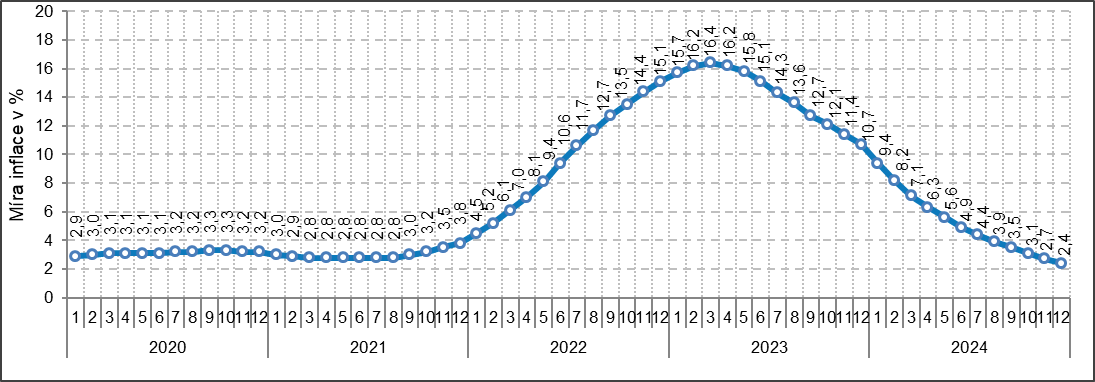
\includegraphics[width=\textwidth]{images/csu-inflace-2026.png}
\end{figure}}

\end{frame}

\begin{frame}{Příklad}{nižší inflace $\neq$ nižší ceny}

    \visible<2->{\begin{talertbox}{Závěr}
    "Inflace v~roce 2024 oproti roku 2023 klesla, takže ceny musely také klesnout."
    \end{talertbox}}

    \visible<3->{\begin{center}
    \obrazek[0.4\textheight]{images/priklad-nizsi-inflace-nizsi-ceny.tex}
    \end{center}}

    \visible<4->{\begin{itemize}
        \item Inflace měří změnu cenové hladiny.
        \visible<5->{\item Pokud je inflace kladná, ceny v~průměru stále rostou.}
        \visible<6->{\item Nižší inflace tedy znamená, že ceny rostou pomaleji než dříve.}
    \end{itemize}}

    \visible<7->{{\scriptsize Zdroj: \url{https://csu.gov.cz/pak/prumerna-rocni-mira-inflace-v-cr-v-roce-2024-byla-24}.}}
\end{frame}

\begin{frame}{Příklad}{Údaj za~celek neplatí pro každou část}

\visible<2->{V~roce 2025 byla podle dat ČSÚ u~voleb do Poslanecké sněmovny Parlamentu České republiky celková účast $68{,}95\,\%$.}

\visible<3->{\begin{talertbox}{Závěr}
    V~Ústeckém kraji z~celkových $632\,844$ oprávněných voličů jich hlasovalo $436\,346$.
\end{talertbox}}

\visible<4->{Výpočet vychází z~předpokladu, že údaj pro celek se nutně vztahuje i~na jeho část:
\[632\,844\cdot 0{,}6895=436\,346.\]}

\visible<5->{\begin{center}
\begin{tabular}{c|c}
\textbf{Území} & \textbf{Volební účast} \\
\hline
Česká republika & $68{,}95\,\%$ \\
Ústecký kraj & $61{,}96\,\%$
\end{tabular}
\end{center}}

\end{frame}

\begin{frame}{Příklad}{Údaj za~celek neplatí pro každou část}

    \visible<2->{\begin{timportantframe}
    Z~údaje za celek nelze bez dalšího odvozovat závěr o~každé jeho části.
    Podmnožiny mohou mít jiné složení, chování i~hodnoty sledovaného znaku.
    \end{timportantframe}}

    \visible<3->{{\scriptsize Zdroje: \cite{csu-volby-snemovna,volby-ps2025}}}

\end{frame}

\subsection{Statistický soubor a~statistický znak}

\begin{frame}{Statistický soubor a~statistický znak}
    \small

    \visible<2->{\begin{defblock}
        \begin{itemize}
            \item \markdarkred{Statistický znak} je sledovaná vlastnost objektů ve statistickém souboru.
            \item \markdarkred{Statistický soubor} s~$n$ objekty a~$p$ sledovanými znaky můžeme chápat jako matici
            \[
            \mathbf{X} =
            \begin{pmatrix}
            x_{11} & x_{12} & \cdots & x_{1p} \\
            x_{21} & x_{22} & \cdots & x_{2p} \\
            \vdots & \vdots & \ddots & \vdots \\
            x_{n1} & x_{n2} & \cdots & x_{np}
            \end{pmatrix}.
            \]
        \end{itemize}
    \end{defblock}}

    \visible<3->{\begin{tnoticeframe}
        Pokud je sledovaný znak pouze jeden, můžeme soubor $\mathbf{X}$ považovat za $n$-rozměrný vektor, tj. $\mathbf{X}=(x_1,\dots,x_n)$.
    \end{tnoticeframe}}    

\end{frame}

\begin{frame}{Statistický soubor a~statistický znak}

    \visible<2->{\begin{itemize}
        \item řádky odpovídají jednotlivým \markdarkred{objektům},
        \visible<3->{\item sloupce odpovídají sledovaným \markdarkred{statistickým znakům},}
        \visible<4->{\item hodnota $x_{ij}$ je hodnota $j$-tého znaku u~$i$-tého objektu.}
    \end{itemize}}

    \visible<5->{\begin{timportantframe}
        My ale budeme typicky pracovat se soubory \textbf{sledující jeden statistický znak}. Resp. jeden sloupec většího souboru budeme považovat za samostatný (pod)soubor.
    \end{timportantframe}}

    \visible<6->{Dále budeme pro statistické soubory $\mathbf{X}=(x_1,\dots,x_n),\mathbf{Y}=(y_1,\dots,y_n)$ a~$a\in\R$ značit
    \begin{itemize}
        \item $\mathbf{X}+\mathbf{Y}=(x_1+y_1,\dots,x_n+y_n)$ a
        \visible<7->{\item $a\mathbf{X}=(ax_1,\dots,ax_n)$.}
    \end{itemize}}
\end{frame}

% =================================================================
\section{Charakteristiky polohy}
% =================================================================

\begin{titleframeenv}{Charakteristiky polohy}
    \obrazek[0.4\textheight]{images/dukaz-bodu-1-i-1-n-x-i-x-0.tex}
\end{titleframeenv}

\subsection{Aritmetický průměr}

\begin{frame}{Aritmetický průměr}

    \begin{defblock}[Aritmetický průměr]
    Mějme statistický soubor $\mathbf{X}=(x_1,\dots,x_n)$. \markdarkred{Aritmetický průměr} $j$-tého statistického znaku definujeme jako
    \[
    \average{\mathbf{X}}_j=\frac{1}{n}\sum_{i=1}^{n}x_{ij}.
    \]
    Je-li statistický znak pouze jeden, můžeme psát jen $\average{\mathbf{X}}$.
    \end{defblock}

    \begin{itemize}
        \item průměrujeme hodnoty v~jednom sloupci,
        \item každá hodnota má stejnou váhu,
        \item průměr nemusí být jednou z~naměřených hodnot.
    \end{itemize}

\end{frame}

\subsection{Vlastnosti aritmetického průměru}

\begin{frame}{Vlastnosti aritmetického průměru}
    \footnotesize

Pro pevně zvolený statistický znak pišme jednoduše
\[
\mathbf{X}=(x_1,x_2,\ldots,x_n)
\qquad\text{a}\qquad
\average{\mathbf{X}}=\frac{1}{n}\sum_{i=1}^{n}x_i.
\]

\begin{propblock}
    Pro statistický soubor $\mathbf{X}$ platí:
    \begin{enumerate}
        \item $\displaystyle \sum_{i=1}^{n}(x_i-\average{\mathbf{X}})=0.$
        \item Pro soubory $\mathbf{X},\mathbf{Y}$ a~čísla $a,b\in\R$ je $\average{a\mathbf{X}+b\mathbf{Y}}=a\average{\mathbf{X}}+b\average{\mathbf{Y}}$.
        \item Aritmetický průměr minimalizuje hodnotu výrazu $\sum_{i=1}^{n}(x_i-a)^2$,
        nebo-li
        \[\average{\mathbf{X}}=\argmin\limits_{a\in\mathbb{R}}\sum_{i=1}^{n}(x_i-a)^2.\]
    \end{enumerate}
\end{propblock}

\end{frame}

\begin{frame}{Důkaz bodu 1}{$\sum_{i=1}^{n}(x_i-\average{\mathbf{X}})=0$}

    \visible<2->{\begin{align*}
        \sum_{i=1}^{n}(x_i-\average{\mathbf{X}})&=\sum_{i=1}^{n}x_i-\sum_{i=1}^{n}\average{\mathbf{X}}=\sum_{i=1}^{n}x_i-n\average{\mathbf{X}}\\
        &=\sum_{i=1}^{n}x_i-n\cdot\frac{1}{n}\sum_{i=1}^{n}x_i=\sum_{i=1}^{n}x_i-\sum_{i=1}^{n}x_i=0.
    \end{align*}}

    \visible<3->{\begin{center}
    \obrazek[0.28\textheight]{images/dukaz-bodu-1-i-1-n-x-i-x-0.tex}
    \end{center}}
\end{frame}

\begin{frame}{Důkaz bodu 2}{$\average{a\mathbf{X}+b\mathbf{Y}}=a\average{\mathbf{X}}+b\average{\mathbf{Y}}$}

    \visible<2->{Soubor $a\mathbf{X}+b\mathbf{Y}$ obsahuje hodnoty
    \[
    ax_1+by_1,\ ax_2+by_2,\ \ldots,\ ax_n+by_n.
    \]}

    \visible<3->{Proto
    \begin{align*}
        \average{a\mathbf{X}+b\mathbf{Y}}&=\frac{1}{n}\sum_{i=1}^{n}(ax_i+by_i)\\
        &=a\cdot\frac{1}{n}\sum_{i=1}^{n}x_i+b\cdot\frac{1}{n}\sum_{i=1}^{n}y_i=a\average{\mathbf{X}}+b\average{\mathbf{Y}}.
    \end{align*}}

\end{frame}

\begin{frame}{Důkaz bodu 3}{minimalizace $\sum_{i=1}^{n}(x_i-a)^2$}
    \footnotesize

\visible<2->{Mějme libovolné $a\in\mathbb{R}$. Pak upravíme:
\[
x_i-a=(x_i-\average{\mathbf{X}})+(\average{\mathbf{X}}-a).
\]}

\visible<3->{Tedy po dosazení, roznásobení a~aplikaci prvního bodu máme:
\begin{align*}
    \sum_{i=1}^{n}(x_i-a)^2&=\sum_{i=1}^{n}\left((x_i-\average{\mathbf{X}})+(\average{\mathbf{X}}-a)\right)^{2}\\
    &=\sum_{i=1}^{n}(x_i-\average{\mathbf{X}})^2+2(\average{\mathbf{X}}-a)\overbrace{\sum_{i=1}^{n}(x_i-\average{\mathbf{X}})}^{0}+n(\average{\mathbf{X}}-a)^2\\
    &=\sum_{i=1}^{n}(x_i-\average{\mathbf{X}})^2+n(\average{\mathbf{X}}-a)^2.
\end{align*}}

\visible<4->{Minimum nastává právě pro $a=\average{\mathbf{X}}$.}

\end{frame}

\subsection{Vážený aritmetický průměr}

\begin{frame}{Vážený aritmetický průměr}


\visible<2->{\begin{defblock}[Vážený aritmetický průměr]
Mějme statistický soubor $\mathbf{X}=(x_1,\ldots,x_n)$ a~vektor \textbf{kladných vah $\mathbf{w}=(w_1,\ldots,w_n)$}. \markdarkred{Vážený aritmetický průměr} definujeme jako
\[
\average{\mathbf{X}}_{\mathbf{w}}
=
\frac{\sum_{i=1}^{n}w_ix_i}{\sum_{i=1}^{n}w_i}.
\]
\end{defblock}}


\visible<3->{\begin{itemize}
    \item Hodnota s~větší vahou má na výsledek větší vliv.
    \item Pokud jsou všechny váhy stejné, tj. $w_1=w_2=\cdots=w_n$, dostaneme obyčejný aritmetický průměr $\average{\mathbf{X}}_\mathbf{w}=\average{\mathbf{X}}$.
\end{itemize}}

\end{frame}

\begin{frame}{Příklad}{Výpočet váženého průměru}
    \small


\visible<2->{Výsledná známka z~předmětu může být určena z~několika částí:

\begin{center}
\begin{tabular}{c|c|c}
\textbf{Část} & \textbf{Výsledek} & \textbf{Váha} \\
\hline
test & $80$ & $2$ \\
projekt & $95$ & $3$ \\
aktivita & $70$ & $1$
\end{tabular}
\end{center}}


\visible<3->{Tedy
\[
\mathbf{X}=(80,95,70),
\qquad
\mathbf{w}=(2,3,1).
\]}


\visible<4->{\[
\average{\mathbf{X}}_{\mathbf{w}}
=
\frac{2\cdot80+3\cdot95+1\cdot70}{2+3+1}
=
\frac{515}{6}
\approx 85{,}83.
\]}


\visible<5->{\begin{tinfoframe}
Projekt má na výsledek větší vliv než aktivita, protože má větší váhu.
\end{tinfoframe}}

\end{frame}

\begin{frame}{Normalizované váhy}



\visible<2->{\begin{propblock}
Mějme váhy
\[
\mathbf{w}=(w_1,\ldots,w_n),
\qquad
w_i>0.
\]
Položme
\[
\omega_i=\frac{w_i}{w_1+\cdots+w_n}.
\]
Potom platí $0<\omega_i\leqslant 1$ pro každé $i\in\set{1,\ldots,n}$,
\[
\omega_1+\cdots+\omega_n=1\quad\text{a}\quad \average{\mathbf{X}}_{\mathbf{w}}
=
\omega_1x_1+\cdots+\omega_nx_n.
\]
\end{propblock}}

\end{frame}

\begin{frame}{Důkaz tvrzení}

    \visible<2->{\begin{itemize}
        \item Skutečnost, že $0<\omega_i\leqslant 1$ je zjevná.
        \visible<3->{\item Počítáním dostaneme:
        \[\sum_{i=1}^{n}\omega_i=\sum_{i=1}^{n}\frac{w_i}{\sum_{i=1}^{n}w_i}=\frac{1}{\sum_{i=1}^{n}w_i}\sum_{i=1}^{n}w_i=1\]}
        \visible<4->{a
        \[\average{\mathbf{X}}_\mathbf{w}=\frac{\sum_{i=1}^{n}w_ix_i}{\sum_{i=1}^{n}w_i}=\sum_{i=1}^{n}\frac{w_i}{\sum_{i=1}^{n}w_i}x_i=\sum_{i=1}^{n}\omega_ix_i.\]}
    \end{itemize}}
\end{frame}

\begin{frame}{Vážený průměr leží mezi hodnotami}



\visible<2->{\begin{propblock}
Pro statistický soubor $\mathbf{X}=(x_1,\ldots,x_n)$ a~kladné váhy
$\mathbf{w}=(w_1,\ldots,w_n)$ platí
\[
\min_{1\leqslant i\leqslant n} x_i
\leqslant
\average{\mathbf{X}}_{\mathbf{w}}
\leqslant
\max_{1\leqslant i\leqslant n} x_i.
\]
\end{propblock}}

\end{frame}

\begin{frame}{Důkaz tvrzení}

    \visible<2->{Označme
    \[
    m=\min_{1\leqslant i\leqslant n} x_i,
    \qquad
    M=\max_{1\leqslant i\leqslant n} x_i.
    \]
    Pak pro každé $i$ platí
    \[
    m\leqslant x_i\leqslant M.
    \]}


    \visible<3->{Protože $\omega_i>0$ a~$\omega_1+\cdots+\omega_n=1$, dostáváme
    \begin{align*}
        \omega_1m+\cdots+\omega_nm&\leqslant\omega_1x_1+\cdots+\omega_nx_n\leqslant\omega_1M+\cdots+\omega_nM,\\
        m(\omega_1+\cdots+\omega_n)&\leqslant\omega_1x_1+\cdots+\omega_nx_n\leqslant M(\omega_1+\cdots+\omega_n).\\
        m &\leqslant\omega_1x_1+\cdots+\omega_nx_n\leqslant M
    \end{align*}}


    \visible<4->{Tedy
    \[
    m
    \leqslant
    \average{\mathbf{X}}_{\mathbf{w}}
    \leqslant
    M.
    \]}
\end{frame}

\subsection{Medián}

\begin{frame}{Medián}
    \footnotesize

\visible<2->{Pro pevně zvolený statistický znak pišme jeho hodnoty jako
\[
x_1,x_2,\ldots,x_n.
\]}
\visible<3->{Po uspořádání vzestupně je označme
\[
x_{(1)}\leqslant x_{(2)}\leqslant \cdots \leqslant x_{(n)}.
\]}

\visible<4->{\begin{defblock}[Medián]
\markdarkred{Medián} souboru $\mathbf{X}$ definujeme jako
\[
\median(\mathbf{X})
=
\begin{cases}
x_{\left((n+1)/2\right)}, & \text{je-li } n \text{ liché},\\[0.2cm]
\frac{x_{\left(n/2\right)}+x_{\left(n/2+1\right)}}{2},
& \text{je-li } n \text{ sudé}.
\end{cases}
\]
\end{defblock}}

\visible<5->{\begin{tinfoframe}
    \begin{center}
        Medián je "prostřední" hodnota uspořádaného souboru.
    \end{center}
\end{tinfoframe}}

\end{frame}

\begin{frame}{Příklad}{Výpočet mediánu}

    \visible<2->{\begin{itemize}
        \item Pro hodnoty statistického znaku
        \[
        3,\ 2,\ 100,\ 5,\ 4\quad\stackrel{\text{seřazení}}{\longrightarrow}\quad 2,\ 3,\ 4,\ 5,\ 100
        \]
        platí $\median(\mathbf{X})=4$.
        \visible<3->{\item Ovšem všimněme si, že
        \[4=\median(\mathbf{X})<\average{\mathbf{X}}=22{,}8.\]}
    \end{itemize}}

    \visible<4->{\begin{talertframe}
        Většina hodnot je \textbf{pod průměrem!} Tento efekt způsobuje hodnota $100$ v~souboru. Takovým hodnotám se říká \markdarkred{odlehlé hodnoty} nebo \markdarkred{odlehlé pozorování}.
    \end{talertframe}}
\end{frame}

% =================================================================
\section{Charakteristiky variability}
% =================================================================

\begin{titleframeenv}{Charakteristiky variability}
    \obrazek[0.4\textheight]{images/maly-a-velky-rozptyl-2.tex}
\end{titleframeenv}

\subsection{Rozptyl}

\begin{frame}{Rozptyl}

\visible<2->{\begin{defblock}[Rozptyl]
Mějme statistický soubor $\mathbf{X}=(x_1,\ldots,x_n)$. \markdarkred{Rozptyl} souboru $\mathbf{X}$ definujeme jako
\[
\Var(\mathbf{X})=\sigma_{\mathbf{X}}^2=\frac{1}{n}\sum_{i=1}^{n}(x_i-\average{\mathbf{X}})^2.
\]
\end{defblock}}

\visible<3->{\begin{itemize}
    \item Anglicky \emph{variance}.
    \item Rozptyl měří, jak moc jsou hodnoty vzdálené od průměru.
    \visible<4->{\item Čím větší je rozptyl, tím více jsou data rozptýlená.}
    \visible<5->{\item Pracujeme se \textbf{čtverci odchylek}, proto je rozptyl vždy nezáporný.}
\end{itemize}}

\visible<6->{\begin{tinfoframe}
Rozptyl je roven nule právě tehdy, když jsou všechny hodnoty stejné.
\end{tinfoframe}}

\end{frame}

\begin{frame}{Malý a~velký rozptyl}

\small

\visible<2->{\begin{columns}[T]
    \begin{column}{0.48\textwidth}
        \begin{center}
            \textbf{Malý rozptyl}
            
            
            \obrazek[0.4\textheight]{images/maly-a-velky-rozptyl-1.tex}
        \end{center}
    \end{column}

    \begin{column}{0.48\textwidth}\visible<3->{
        \begin{center}
            \textbf{Velký rozptyl}
            
            
            \obrazek[0.4\textheight]{images/maly-a-velky-rozptyl-2.tex}
        \end{center}
    }\end{column}
\end{columns}}

\visible<3->{\vspace{0.15cm}}

\visible<4->{\begin{timportantframe}
V~obou případech je průměr stejný, ale ve druhém souboru jsou hodnoty
od průměru vzdálenější, a~proto $\Var(\mathbf{X})<\Var(\mathbf{Y})$.
\end{timportantframe}}

\end{frame}

\begin{frame}{Příklad}{Výpočet rozptylu}
    \small

\visible<2->{Během pěti dnů jsme naměřili polední teploty ve stupních Celsia:
\[
\mathbf{T}=(18,20,20,21,26).
\]}

\visible<3->{Pak spočítáme:
\begin{align*}
    \average{\mathbf{T}}&=\frac{18+20+20+21+26}{5}=21,\\
    \Var(\mathbf{T})&=\frac{1}{5}\left((18-21)^2+(20-21)^2+(20-21)^2+(21-21)^2+(26-21)^2\right)\\
    &=\boxed{7{,}2}.
\end{align*}}

\visible<4->{\begin{tinfoframe}
Rozptyl teplot je $7{,}2\,^\circ\mathrm{C}^2$.
Vyšší hodnota je způsobena hlavně dnem s~teplotou $26\,^\circ\mathrm{C}$.
\end{tinfoframe}}

\end{frame}

\subsection{Směrodatná odchylka}

\begin{frame}{Směrodatná odchylka}

\visible<2->{\begin{defblock}[Směrodatná odchylka]
Mějme statistický soubor $\mathbf{X}=(x_1,\ldots,x_n)$. \markdarkred{Směrodatnou odchylku} statistického souboru $\mathbf{X}$ definujeme jako
\[
\sigma_{\mathbf{X}}=\sqrt{\Var(\mathbf{X})}=\sqrt{\frac{1}{n}\sum_{i=1}^{n}(x_i-\average{\mathbf{X}})^2}.
\]
\end{defblock}}

\visible<3->{\begin{exblock}
    Z~minulého příkladu můžeme určit, že
    \[\sigma_\mathbf{T}=\sqrt{\Var(\mathbf{T})}=\sqrt{7{,}2}\approx 2{,}683\,^\circ\mathrm{C}\]
\end{exblock}}

\end{frame}

\subsection{Vztah průměru, mediánu a~směrodatné odchylky}

\begin{frame}{Vztah průměru, mediánu a~směrodatné odchylky}

\visible<2->{\begin{propblock}[Bez důkazu]
Pro libovolný statistický soubor $\mathbf{X}=(x_1,\dots,x_n)$ platí
\[
\left|\average{\mathbf{X}}-\median(\mathbf{X})\right|\leqslant\sigma_{\mathbf{X}}.
\]
\end{propblock}}

\visible<3->{\begin{itemize}
    \item Obecně nelze říci, zda je větší průměr nebo medián.
    \visible<4->{\item Jejich vzdálenost je ale omezena směrodatnou odchylkou.}
    \visible<5->{\item Pokud jsou průměr a~medián daleko od sebe, data mají \textbf{velký rozptyl}.}
\end{itemize}}

\visible<6->{\begin{tinfoframe}
Směrodatná odchylka tedy říká i~to, jak daleko od sebe mohou být různé způsoby popisu "středu" dat.
\end{tinfoframe}}

\end{frame}

% =================================================================
\section{Standardizace dat}
% =================================================================

\begin{titleframeenv}{Standardizace dat}
    \obrazek[0.4\textheight]{images/standardizace-dat-schematicky.tex}
\end{titleframeenv}

\subsection{Standardizovaná hodnota a~soubor}

\begin{frame}{Standardizovaná hodnota a~soubor}


\visible<2->{\begin{defblock}[Standardizovaná hodnota]
Mějme statistický soubor $\mathbf{X}=(x_1,\ldots,x_n)$, kde $\sigma_{\mathbf{X}}>0$.
\markdarkred{Standardizovanou hodnotu} $x_i$ definujeme jako
\[
z_i=\frac{x_i-\average{\mathbf{X}}}{\sigma_{\mathbf{X}}}.
\]
Standardizovaný soubor hodnot značíme $\mathbf{Z}=(z_1,\ldots,z_n)$.
\end{defblock}}


\visible<3->{\begin{tinfoframe}
    Hodnota $z_i$ v~podstatě říká, o~kolik směrodatných odchylek $\sigma_\mathbf{X}$ je~$x_i$ vzdálena od průměru $\average{\mathbf{X}}$.
\end{tinfoframe}}

\end{frame}

\begin{frame}{Standardizace dat schématicky}


\visible<2->{\begin{center}
\obrazek[0.4\textheight]{images/standardizace-dat-schematicky.tex}
\end{center}}


\visible<3->{\begin{timportantframe}
Standardizace posune průměr do nuly a~změní měřítko tak, aby jedna jednotka odpovídala jedné směrodatné odchylce.
\end{timportantframe}}

\end{frame}

\subsection{Vlastnosti standardizovaných dat}

\begin{frame}{Vlastnosti standardizovaných dat}

\small

\visible<2->{\begin{propblock}
Mějme statistický soubor $\mathbf{X}=(x_1,\ldots,x_n)$, kde $\sigma_{\mathbf{X}}>0$.
Pro standardizovaný soubor $\mathbf{Z}$ platí $\average{\mathbf{Z}}=0$ a~$\sigma_{\mathbf{Z}}=1$.
\end{propblock}}


\visible<3->{\textbf{Důkaz.}

\[
\average{\mathbf{Z}}
=
\frac{1}{n}\sum_{i=1}^{n}z_i
=
\frac{1}{n}\sum_{i=1}^{n}
\frac{x_i-\average{\mathbf{X}}}{\sigma_{\mathbf{X}}}
=
\frac{1}{\sigma_{\mathbf{X}}}
\cdot
\frac{1}{n}
\sum_{i=1}^{n}(x_i-\average{\mathbf{X}})
=
0.
\]}


\visible<4->{Protože $\average{\mathbf{Z}}=0$, dostáváme
\[
\Var(\mathbf{Z})
=
\frac{1}{n}\sum_{i=1}^{n}z_i^2
=
\frac{1}{n}\sum_{i=1}^{n}
\left(
\frac{x_i-\average{\mathbf{X}}}{\sigma_{\mathbf{X}}}
\right)^2
=
\frac{1}{\sigma_{\mathbf{X}}^2}
\cdot
\Var(\mathbf{X})
=
\frac{1}{\Var(\mathbf{X})}
\cdot
\Var(\mathbf{X})
=
1.
\]}


\visible<5->{Tedy $\sigma_{\mathbf{Z}}=\sqrt{\Var(\mathbf{Z})}=1$.}

\end{frame}

\begin{frame}{Proč standardizujeme data?}


\visible<2->{Různé statistické znaky mohou mít \markdarkred{různé jednotky} a~\markdarkred{různé měřítko}.}


\visible<3->{\begin{exblock}
Například u~jednoho člověka můžeme sledovat:
\[
\text{věk}=18\text{ let},
\qquad
\text{příjem}=35\,000\text{ Kč}.
\]
\end{exblock}}


\visible<4->{\begin{itemize}
    \item Bez úpravy může znak s~většími čísly působit "důležitěji".
    \visible<5->{\item Standardizace převede hodnoty na společné měřítko.}
    \visible<6->{\item Hodnoty pak říkají, o~kolik směrodatných odchylek se liší od průměru.}
\end{itemize}}


\visible<7->{\begin{timportantframe}
Standardizace pomáhá porovnávat různé statistické znaky
a~připravit data pro některé metody umělé inteligence.
\end{timportantframe}}

\end{frame}

\begin{frame}{Příklad}{věk a~příjem}

\begin{center}
\begin{tabular}{c|c|c}
\textbf{Osoba} & \textbf{Věk} & \textbf{Příjem} \\
\hline
1 & 18 & $22\,000$ Kč \\
2 & 22 & $28\,000$ Kč \\
3 & 25 & $31\,000$ Kč \\
4 & 31 & $38\,000$ Kč \\
5 & 35 & $45\,000$ Kč \\
6 & 40 & $52\,000$ Kč \\
7 & 46 & $61\,000$ Kč \\
8 & 52 & $69\,000$ Kč \\
9 & 58 & $78\,000$ Kč \\
10 & 65 & $90\,000$ Kč
\end{tabular}
\end{center}

\end{frame}

\begin{frame}{Příklad}{standardizovaný soubor}

\small

\begin{center}
\begin{tabular}{c|c|c}
\textbf{Osoba} & \textbf{Věk} & \textbf{Příjem} \\
\hline
1 & $-1{,}41$ & $-1{,}36$ \\
2 & $-1{,}14$ & $-1{,}09$ \\
3 & $-0{,}94$ & $-0{,}95$ \\
4 & $-0{,}55$ & $-0{,}62$ \\
5 & $-0{,}28$ & $-0{,}30$ \\
6 & $0{,}05$ & $0{,}03$ \\
7 & $0{,}45$ & $0{,}45$ \\
8 & $0{,}85$ & $0{,}82$ \\
9 & $1{,}25$ & $1{,}23$ \\
10 & $1{,}72$ & $1{,}79$
\end{tabular}
\end{center}

\begin{tinfoframe}
Po standardizaci už hodnoty ve sloupcích \textbf{věk} a~\textbf{příjem}
nejsou v~tak rozdílném měřítku.
\end{tinfoframe}

\end{frame}

% =================================================================
\section{Min-max normalizace dat}
% =================================================================

\begin{titleframeenv}{Min-max normalizace dat}
    \obrazek[0.4\textheight]{images/dvojice-hodnot-a-bodovy-graf.tex}
\end{titleframeenv}

\begin{frame}{Min-max normalizace}
    \footnotesize


\visible<2->{\begin{defblock}[Min-max normalizace]
Mějme statistický soubor $\mathbf{X}=(x_1,\ldots,x_n)$ a~označme
\[
m=\min_i x_i,\qquad M=\max_i x_i.
\]
Je-li $M>m$, definujeme min-max normalizované hodnoty jako
\[
u_i=\frac{x_i-m}{M-m}.
\]
\end{defblock}}


\visible<3->{\begin{itemize}
    \item Nejmenší hodnota se zobrazí na~$0$.
    \item Největší hodnota se zobrazí na~$1$.
    \item Všechny ostatní hodnoty leží mezi nimi.
\end{itemize}}


\visible<4->{\begin{timportantframe}
Min-max normalizace převádí data do intervalu $\langle 0,1\rangle$.
\end{timportantframe}}

\end{frame}

\begin{frame}{Příklad}{Min-max normalizace}
    \small


\visible<2->{Použijme opět soubor poledních teplot:
\[
\mathbf{T}=(18,20,20,21,26).
\]}


\visible<3->{Platí
\[
m=18,\qquad M=26,\qquad M-m=8.
\]}


\visible<4->{\[
\begin{aligned}
    \mathbf{U}
    &=
    \left(
    \frac{18-18}{8},
    \frac{20-18}{8},
    \frac{20-18}{8},
    \frac{21-18}{8},
    \frac{26-18}{8}
    \right)\\
    &=(0;\ 0{,}25;\ 0{,}25;\ 0{,}375;\ 1).
\end{aligned}
\]}


\visible<5->{\begin{tinfoframe}
Původní teploty ve~stupních Celsia jsme převedli na~bezrozměrné hodnoty
v~intervalu $\langle 0,1\rangle$.
\end{tinfoframe}}

\end{frame}

% =================================================================
\section{Korelace}
% =================================================================

\begin{titleframeenv}{Korelace}
    \obrazek[0.4\textheight]{images/vyznam-hodnot-korelace-1.tex}
\end{titleframeenv}

\subsection{Dva statistické znaky}

\begin{frame}{Dva statistické znaky}


\visible<2->{Dosud jsme pracovali hlavně s~jedním statistickým znakem.}


\visible<3->{\begin{tinfoframe}
Někdy nás ale zajímá, zda spolu dva statistické znaky nějak souvisí.
\end{tinfoframe}}


\visible<4->{Například:
\begin{itemize}
    \item výška a~hmotnost,
    \item vzdělání a~příjem,
    \item teplota a~prodej zmrzliny.
\end{itemize}}


\visible<5->{\begin{timportantframe}
Cílem není pouze popsat jednotlivé znaky zvlášť, ale zjistit, zda mezi nimi existuje nějaký vztah.
\end{timportantframe}}

\end{frame}

\begin{frame}{Dvojice hodnot a~bodový graf}


\visible<2->{Mějme dva statistické soubory
\[
\mathbf{X}=(x_1,\ldots,x_n),
\qquad
\mathbf{Y}=(y_1,\ldots,y_n).
\]}


\visible<3->{Hodnoty uspořádáme do dvojic
\[
(x_1,y_1),\ (x_2,y_2),\ \ldots,\ (x_n,y_n).
\]}


\visible<4->{\begin{columns}[T]
    \begin{column}{0.48\textwidth}
        \begin{center}
        \obrazek[0.28\textheight]{images/dvojice-hodnot-a-bodovy-graf.tex}
        \end{center}
    \end{column}

    \begin{column}{0.48\textwidth}\visible<5->{
        \vspace{1cm}
        \begin{tinfoframe}
        Bodový graf často rychle ukáže, zda mezi dvěma znaky může být vztah.
        \end{tinfoframe}
    }\end{column}
\end{columns}}

\end{frame}

\subsection{Kovariance}

\begin{frame}{Kovariance}
    \footnotesize


\visible<2->{\begin{defblock}[Kovariance]
Mějme statistické soubory $\mathbf{X}=(x_1,\ldots,x_n),\mathbf{Y}=(y_1,\ldots,y_n)$. \markdarkred{Kovarianci} souborů $\mathbf{X}$ a~$\mathbf{Y}$ definujeme jako
\[
\Cov(\mathbf{X},\mathbf{Y})
=
\frac{1}{n}\sum_{i=1}^{n}
(x_i-\average{\mathbf{X}})(y_i-\average{\mathbf{Y}}).
\]
\end{defblock}}


\visible<3->{\begin{itemize}
    \item Lze ihned vidět, že $\Cov(\mathbf{X},\mathbf{X})=\Var(\mathbf{X})$.
    \visible<4->{\item Kladná kovariance: větší hodnoty $\mathbf{X}$ často odpovídají větším hodnotám $\mathbf{Y}$.}
    \visible<5->{\item Záporná kovariance: větší hodnoty $\mathbf{X}$ často odpovídají menším hodnotám $\mathbf{Y}$.}
\end{itemize}}

\visible<6->{\begin{talertbox}{Problém}
    \begin{center}
        Kovariance závisí na jednotkách a~"měřítku" dat.
    \end{center}
\end{talertbox}}

\end{frame}

\subsection{Korelační koeficient}

\begin{frame}{Korelační koeficient}
    \small


\visible<2->{\begin{defblock}[Korelační koeficient]
Mějme statistické soubory $\mathbf{X}$ a~$\mathbf{Y}$, kde
$\sigma_{\mathbf{X}}>0$ a~$\sigma_{\mathbf{Y}}>0$.
\markdarkred{Korelační koeficient} definujeme jako
\[
\rho_{\mathbf{X}\mathbf{Y}} 
=
\frac{\Cov(\mathbf{X},\mathbf{Y})}
{\sigma_{\mathbf{X}}\sigma_{\mathbf{Y}}}.
\]
\end{defblock}}


\visible<3->{Ekvivalentně:
\[
\rho_{\mathbf{X}\mathbf{Y}}
=
\frac{
\sum_{i=1}^{n}(x_i-\average{\mathbf{X}})(y_i-\average{\mathbf{Y}})
}{
\sqrt{\sum_{i=1}^{n}(x_i-\average{\mathbf{X}})^2}
\sqrt{\sum_{i=1}^{n}(y_i-\average{\mathbf{Y}})^2}
}=\frac{1}{n\sigma_\mathbf{X}\sigma_\mathbf{Y}}\left(\sum_{i=1}^{n}x_iy_i-n\average{\mathbf{X}}\average{\mathbf{Y}}\right).
\]}


\visible<4->{\begin{tinfoframe}
Korelační koeficient je standardizovaná kovariance. Nemá jednotky a~měří míru \markdarkred{lineární závislosti}.
\end{tinfoframe}}

\end{frame}

\subsection{Význam hodnot korelace}

\begin{frame}{Význam hodnot korelace}


\visible<2->{\begin{columns}[T]
\begin{column}{0.32\textwidth}
\centering
\textbf{Kladná korelace}
\vspace{0.1cm}
\begin{center}
    \obrazek[0.4\textheight]{images/vyznam-hodnot-korelace-1.tex}
\end{center}
\end{column}


\begin{column}{0.32\textwidth}\visible<3->{
\centering
\textbf{Záporná korelace}
\vspace{0.1cm}
\begin{center}
    \obrazek[0.4\textheight]{images/vyznam-hodnot-korelace-2.tex}
\end{center}
}\end{column}


\begin{column}{0.32\textwidth}\visible<4->{
\centering
\textbf{Bez lin. korelace}
\vspace{0.1cm}
\begin{center}
    \obrazek[0.4\textheight]{images/vyznam-hodnot-korelace-3.tex}
\end{center}
}\end{column}
\end{columns}}


\visible<5->{\vspace{0.3cm}

\begin{timportantframe}
Korelace měří směr a~sílu \textbf{lineárního} vztahu mezi dvěma znaky.
\end{timportantframe}}

\end{frame}

\subsection{Vlastnosti korelačního koeficientu}

\begin{frame}{Vlastnosti korelačního koeficientu}


\visible<2->{\begin{propblock}[Bez důkazu]
    Pro korelační koeficient souborů $\mathbf{X},\mathbf{Y}$ platí
    \begin{enumerate}
        \item $-1\leqslant \rho_{\mathbf{X}\mathbf{Y}}\leqslant 1$,
        \item $\rho_{\mathbf{X}\mathbf{Y}}=\pm 1$ právě tehdy, když $\mathbf{Y}=\alpha\mathbf{X}+\beta$ pro vhodná $\alpha,\beta\in\R$, $\alpha\neq 0$.
    \end{enumerate}
\end{propblock}}


\visible<3->{\begin{itemize}
    \item $\rho_{\mathbf{X}\mathbf{Y}}=1$ znamená dokonalou \markdarkred{kladnou lineární závislost}.
    \item $\rho_{\mathbf{X}\mathbf{Y}}=-1$ znamená dokonalou \markdarkred{zápornou lineární závislost}.
    \item $\rho_{\mathbf{X}\mathbf{Y}}=0$ znamená, že mezi daty \markdarkred{není lineární korelace}.
\end{itemize}}


\visible<4->{\begin{talertbox}{Pozor!}
Hodnota $\rho_{\mathbf{X}\mathbf{Y}}=0$ neznamená nutně,
že mezi znaky není žádný vztah.
Znamená pouze, že mezi nimi není lineární korelace.
\end{talertbox}}

\end{frame}

\begin{frame}{Příklad}{Výška a~hmotnost}

    \footnotesize

    \visible<2->{Mějme data osmi studentů:

    \begin{center}
    \begin{tabular}{c|cccccccc}
    \textbf{Výška [cm]} & 166 & 188 & 175 & 176 & 169 & 181 & 172 & 160 \\
    \hline
    \textbf{Hmotnost [kg]} & 55 & 90 & 53 & 52 & 63 & 76 & 68 & 50
    \end{tabular}
    \end{center}}


    \visible<3->{Označme
    \begin{align*}
        \mathbf{V}&=(166,188,175,176,169,181,172,160),\\
        \mathbf{H}&=(55,90,53,52,63,76,68,50).
    \end{align*}}

    \visible<4->{Po výpočtu dostaneme přibližně:
    \[
    \average{\mathbf{V}}\approx 173{,}38\;;
    \quad
    \average{\mathbf{H}}\approx 63{,}38\;;
    \quad
    \sigma_{\mathbf{V}}\approx 8{,}18\;;
    \quad
    \sigma_{\mathbf{H}}\approx 13{,}11.
    \]}


    \visible<5->{Celkově vychází $\rho_{\mathbf{V}\mathbf{H}}\approx 0{,}79$.}


    \visible<6->{\begin{tinfoframe}
    Mezi výškou a~hmotností je v~tomto malém souboru \textbf{silná kladná lineární korelace}.
    \end{tinfoframe}}

\end{frame}

\begin{frame}{Korelace měří lineární vztah}


    \visible<2->{\begin{center}
    \obrazek[0.4\textheight]{images/korelace-meri-linearni-vztah.tex}
    \end{center}}


    \visible<3->{\begin{talertbox}{Pozor}
    Data mohou být zjevně závislá, ale korelační koeficient může být blízký nule.
    \end{talertbox}}


    \visible<4->{\begin{timportantframe}
    Korelační koeficient zachycuje pouze \textbf{lineární} závislost.
    Nelineární vztahy může snadno "přehlédnout".
    \end{timportantframe}}

\end{frame}

\begin{frame}{Příklad}{Nelineární vztah s~nulovou korelací}
    \small


    \visible<2->{\begin{itemize}
        \item Mějme statistické soubory
        \[
        \mathbf{X}=(x_1,\ldots,x_n),\quad\mathbf{Y}=(y_1,\ldots,y_n),
        \]
        kde $y_i=x_i^2$ pro každé $i$, neboli $\mathbf{Y}=\mathbf{X}^{2}$.
        \visible<3->{\item Předpokládejme navíc, že hodnoty $x_i$ jsou symetrické kolem nuly, tedy pro každé $x_i$ je v~souboru $\mathbf{X}$ i~hodnota $-x_i$.
        \item Z~toho ihned plyne, že $\average{\mathbf{X}}=0$ a~$\sum_{i=1}^{n}x_i^{3}=0$.}
    \end{itemize}}

    \visible<4->{Kovariance tedy vychází nulová:
    \begin{align*}
        \Cov(\mathbf{X},\mathbf{Y})&=\frac{1}{n}\sum_{i=1}^{n}(x_i-\average{\mathbf{X}})(y_i-\average{\mathbf{Y}})=\frac{1}{n}\left(\sum_{i=1}^{n}x_i^{3}-\average{\mathbf{Y}}\sum_{i=1}^{n}x_i\right)\\
        &=\frac{1}{n}\left(0-\average{\mathbf{Y}}\cdot 0\right)=0.
    \end{align*}}


    \visible<5->{Pokud navíc $\sigma_{\mathbf{X}}>0$ a~$\sigma_{\mathbf{Y}}>0$, pak $\rho_{\mathbf{X}\mathbf{Y}}=0$.}

\end{frame}

\subsection{Jak měřit jiné typy závislosti?}

\begin{frame}{Jak měřit jiné typy závislosti?}



\visible<2->{Korelační koeficient není jediný způsob, jak zkoumat vztah mezi daty.}


\visible<3->{\begin{itemize}
    \item \textbf{Transformace dat:}
    pokud čekáme kvadratický vztah, můžeme zkoumat korelaci mezi
    \[
    \mathbf{X}^2
    \quad\text{a}\quad
    \mathbf{Y}.
    \]
    Například pro $\mathbf{Y}=\mathbf{X}^2$ dostaneme
    \[
    \rho_{\mathbf{X}^2\mathbf{Y}}=1.
    \]


    \visible<4->{\item \textbf{Regresní modely:}
    místo přímky lze hledat například parabolu, kubickou funkci nebo exponenciálu:
    \[
    y=ax^2+bx+c,
    \qquad
    y=ae^{bx}.
    \]}


    \visible<5->{\item \textbf{Jiné koeficienty závislosti:}
    pro pořadové nebo monotónní vztahy se používají např. Spearmanův
    nebo Kendallův korelační koeficient.}
\end{itemize}}

\end{frame}

\subsection{Korelace není kauzalita}

\begin{frame}{Korelace není kauzalita}
    \footnotesize


\visible<2->{\begin{tinfoframe}
Korelace znamená, že dvě veličiny se v~datech "mění společně".
Kauzalita znamená, že \markdarkred{jedna veličina je příčinou změny druhé}.
\end{tinfoframe}}


\visible<3->{\[
\text{korelace}
\quad\not\Rightarrow\quad
\text{kauzalita}
\]}


\visible<4->{\begin{exblock}
V~létě roste prodej zmrzliny a~zároveň počet případů úpalu.
\end{exblock}}


\visible<5->{\begin{talertbox}{Chybný závěr}
Zmrzlina způsobuje úpal.
\end{talertbox}}


\visible<6->{\begin{timportantframe}
Obě veličiny mohou růst kvůli třetí proměnné:
například kvůli vyšší teplotě.
\end{timportantframe}}

\end{frame}

\zdrojeframe{russell-norvig-aima, james-isl-python, csu-volby-snemovna, volby-ps2025}

\end{document}